\documentclass[8pt, t,
aspectratio=169,% for widescreen (16:9) presentations
%aspectratio=43,% for traditional (4:3) presentations
]{beamer}
\graphicspath{{fig/}}

%handout%
\usepackage{comment}
\usepackage{bm}
\usepackage{standalone}


%%%%%%%%%%%%%%%%%%%%%%%%%%%%%%%%%% mode options %%%%%%%%%%%%%%%%%%%%%%%%%%%%%%%%

\mode<presentation>{\usetheme{uniS}}

% define a few pictures used throughout the slides
\pgfdeclareimage[height=1.1\paperheight]{background}{./design/bg.jpg}  % background picture for title slide
\pgfdeclareimage[height=1cm]{unilogo}{./design/unistuttgart_ipvs_ac_english_black.pdf} % UniS logo for title slide
\pgfdeclareimage[height=1cm]{unilogow}{./design/unistuttgart_english_white.pdf} % (white) UniS logo for final slide
\pgfdeclareimage[width=2.5cm]{speaker}{./design/speaker.jpeg} % speaker photo for final slide
\pgfdeclareimage[width=1.25cm]{institutelogo}{./design/ac_logo_blue.pdf}


%%%%%%%%%%%%%%%%%%%%%%%%%%%%%%%%%% misc stuff %%%%%%%%%%%%%%%%%%%%%%%%%%%%%%%%%%
\usepackage{multicol}
% automatically display \sectionpage at beginning of every \section{}
\AtBeginSection[]{%
\begin{frame}[plain]
  \sectionpage
\end{frame}

% TODO style needs to be adopted to the subsection slide in PowerPoint
% \AtBeginSubsection[]{
%   \begin{frame}[plain]
%     \subsectionpage    
%   \end{frame}
% }

% % Dont know what this is good for
% % uncomment block in order to display toc after every sectionpage

% \begin{frame}[c, plain]
%  \begin{footnotesize}
%     \begin{center}
%      \begin{minipage}{.75\textwidth}
%         \begin{multicols}{2}
%          \tableofcontents[currentsection]
%         \end{multicols}
%      \end{minipage}
%     \end{center}
%  \end{footnotesize}
% \end{frame}
}
\usetikzlibrary{matrix,shapes,arrows,positioning,chains,patterns,fit,decorations.pathreplacing,calc,plotmarks}
\tikzset{
    dotted_block/.style={
        draw=black!30!white, 
        dashed,
        inner ysep=2mm,
        inner xsep=10mm, 
        rectangle, 
        rounded corners
    },
    block/.style={
        draw,
        rectangle,
        rounded corners,
        minimum height=2em,
        minimum width=2em
    },
    operator/.style={
        draw,
        circle,
        thin,
        minimum height=1em,
	   inner sep=1pt
    },
    weight/.style={
        draw,
        thin,
        rounded corners,
        rectangle,
        %minimum height=2em,
        %minimum width=4em
    },
    value/.style={
        draw,
        thin,
        rectangle,
        %minimum height=2em,
        %minimum width=3em
    },
    gain/.style={
        regular polygon, 
        regular polygon sides=3,
        draw, 
        fill=white, 
        text width=1em,
        inner sep=1mm, 
        outer sep=0mm,
        shape border rotate=-90
    },
    concat/.style={
        draw,
        shape=circle, 
        fill=black,
        %minimum height=0.5em,
	   inner sep=0pt
    },
}

\newcommand{\matr}[1]{\bm{#1}} % matrix
\newcommand{\vect}[1]{\bm{#1}} % vector
\newcommand{\deriv}[1]{\dot{\vect{#1}}} % derivative of vector (dot-notation)
\newcommand{\force}[1]{\vect{\tau}_{\text{#1}}} % force vector
\newcommand{\rb}[0]{\mathit{RB}} % rigid-body abbreviation
\newcommand{\abs}[1]{\lvert #1 \rvert} % abs(x)


%%%%%%%%%%%%%%%%%%%%%%%%%%%%%%%%%%%% setup %%%%%%%%%%%%%%%%%%%%%%%%%%%%%%%%%%%%%

\title[\Acrfull{deq}]{ML in the Science \\ Deep Equilibrium Models}
% \subtitle{Hauptseminar Winterterm 2021}
\author[]{Daniel Frank}
\institute[Analytic Computing]{Institute for Parallel and Distributed Systems}
\date{\today}
%\institute[IPVS]{\inst{1}Institute for Parallel and Distributed Systems\and\inst{2}Analytic Computing}

%%%%%%%%%%%%%%%%%%%%%%%%%%%%%%%%%%% slides %%%%%%%%%%%%%%%%%%%%%%%%%%%%%%%%%%%%%

% ------------------------------------------------------------------------------
% Listings

% In the following we make listings look like algorithms.
% See: https://tex.stackexchange.com/a/73396/75225
\definecolor{acGray}{HTML}{3E444C}
\colorlet{acComment}{acGray!75}
\lstset{
    frame=tb,
    basicstyle=\ttfamily,
    mathescape,
    showstringspaces=false,
    commentstyle=\color{acComment},
    numberstyle=\footnotesize\color{acComment},
    aboveskip=0.4cm,
    belowskip=0.2cm}

\lstdefinestyle{numbered}{
    numbers=left,
    numbersep=4pt,
    xleftmargin=16.5pt,
    framexleftmargin=16.5pt}

\DeclareCaptionFormat{lstlisting}{\hrule\vspace{2pt}#1#2#3}
\captionsetup[lstlisting]{format=lstlisting, singlelinecheck=off}

% ------------------------------------------------------------------------------

\begin{document}

% helpful for blockdiagrams
\tikzstyle{block} = [draw, rectangle, rounded corners, minimum height=2em, minimum width=2em]
\tikzstyle{sum} = [draw, circle]
\tikzstyle{input} = [coordinate]
\tikzstyle{output} = [coordinate]
\tikzstyle{pinstyle} = [pin edge={to-,thin,black}]
\tikzstyle{rect_grey} = [rectangle, fill=black!20, rounded corners=5pt, minimum width = 8cm, minimum height = 1cm]
\tikzstyle{rect_grey_small} = [rectangle, fill=black!10, rounded corners=5pt, minimum width = 4cm, minimum height = 4cm]
% boxes used for topics
\tikzstyle{rect_grey_topic} = [rectangle, fill=black!20, rounded corners=5pt, minimum width = 2cm, minimum height = 1.5cm, align=center]
\tikzstyle{rect_white_topic} = [rectangle, draw, rounded corners=5pt, minimum width = 2cm, minimum height = 1.5cm]

\begin{frame}[plain]
  \titlepage
\end{frame}

% TODO fix table of content, could be a problem with enumerate
\begin{frame}{Outline}
  \tableofcontents
\end{frame}


\section{What are \acrlong{deq}?}
\begin{frame}{\Acrlong{deq} in Machine Learning}
    \framesubtitle{Where do they come from?}
    \begin{columns}[T]
        \column{0.33\textwidth}
            \begin{figure}
                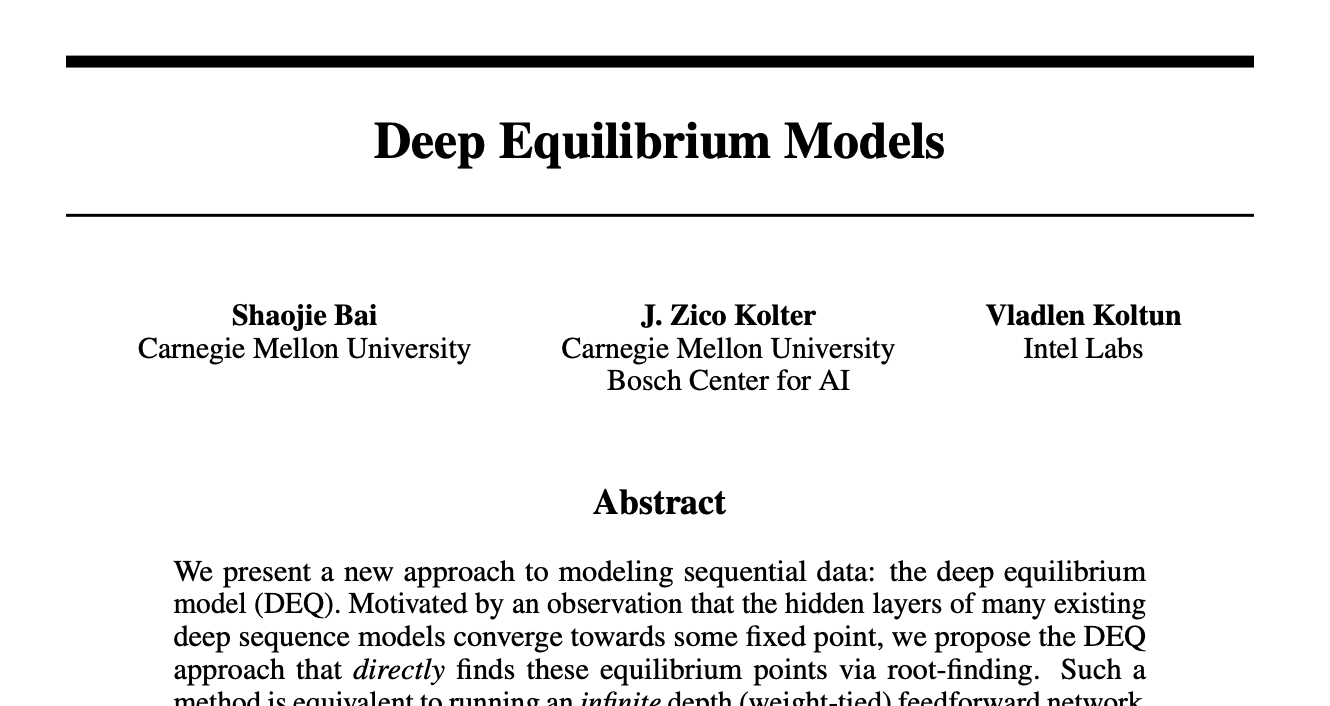
\includegraphics[width=\textwidth]{deq.png}
                \caption{From NeurIPS 2019, \emph{about 400 citations} \cite{bai2019deep}}
            \end{figure}
            \pause
        \column{0.33\textwidth}
            \begin{figure}
                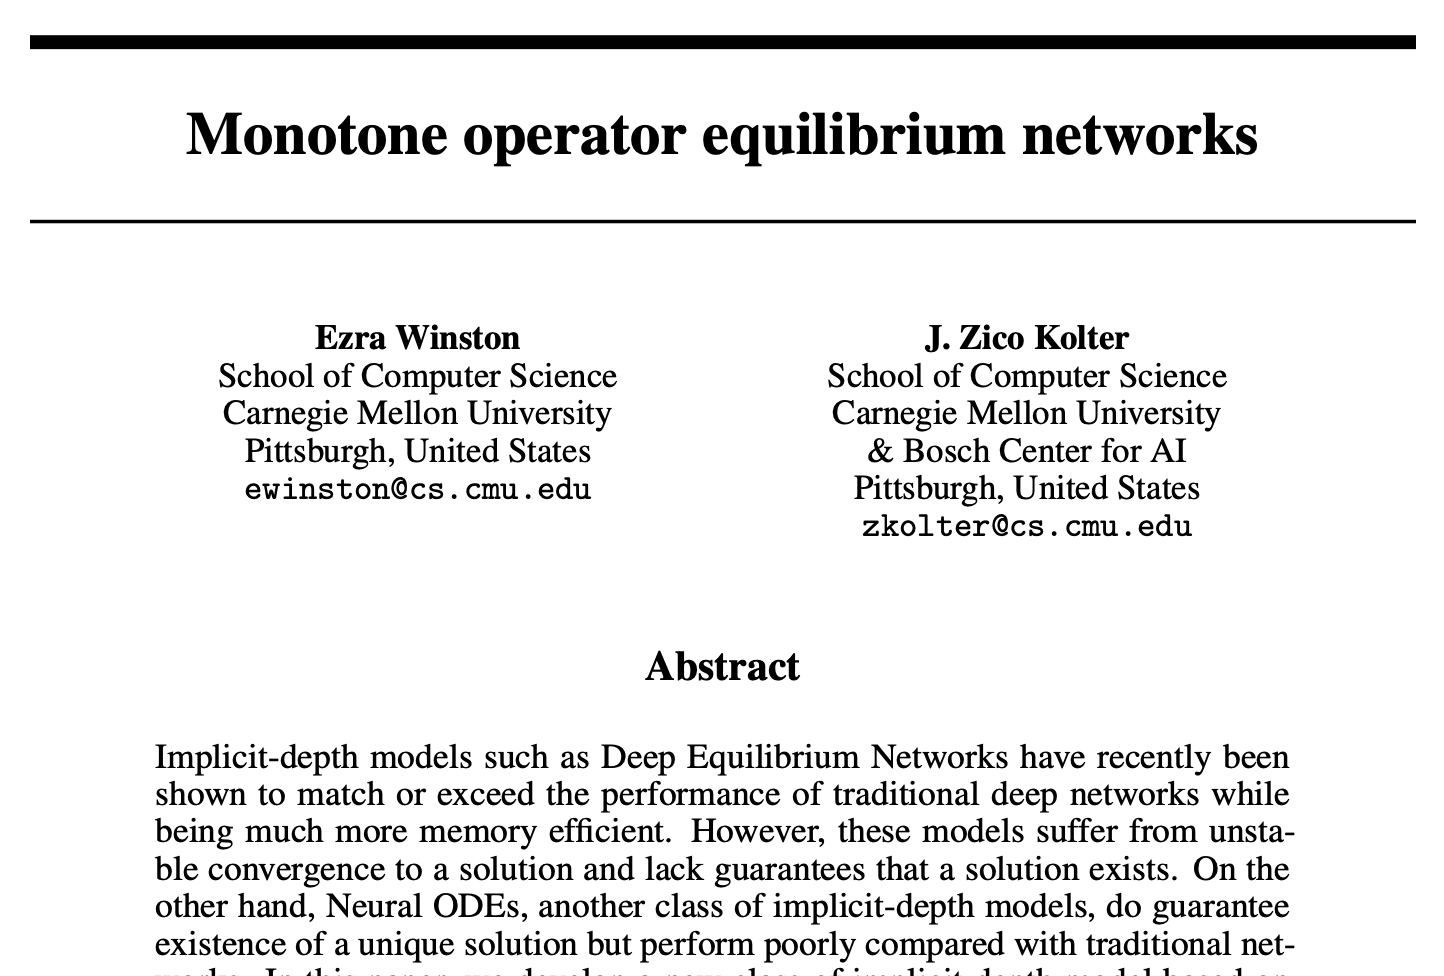
\includegraphics[width=\textwidth]{mon_deq.png}
                \caption{From NeurIPS 2020, \emph{about 70 citations} \cite{winston2020monotone}}
            \end{figure}
            \pause
        \column{0.33\textwidth}
            \begin{figure}
                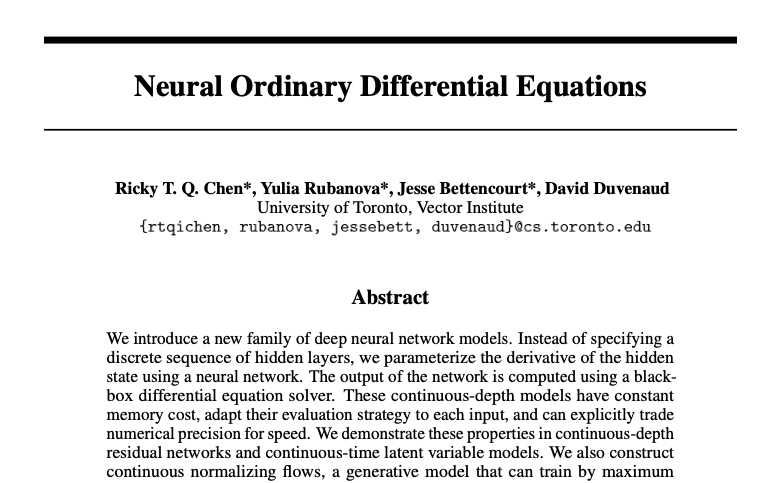
\includegraphics[width=\textwidth]{node.png}
                \caption{From NeurIPS 2018, \emph{about 2700 citations} \cite{chen2018neural} }
            \end{figure}
    \end{columns}
    \pause
    % \begin{block}{Connection between recurrent neural networks and \gls{lti} systems}
    %     \begin{itemize}
    %         \item Recurrent neural networks are a special case of LTI systems with a nonlinear disturbance
    %         \item Equilibrium networks further generalize the network structure
    %         \item Robustness analysis known from robust control can be applied to such systems
    %     \end{itemize}
        
    % \end{block}
    \begin{block}{Why are they interesting?}
        \begin{itemize}
            \item Training of \gls{deq} only requires constant memory
            \item Achieve state-of-the-art performance compared to standard deep learning approaches
            \item \Gls{deq} have a strong relation to system theory
        \end{itemize}
    \end{block}
\end{frame}

\subsection{Forward Pass}
\begin{frame}{\Acrlongpl{deq} - Forward Pass}
    \framesubtitle{\cite{bai2019deep}}

    \begin{itemize}
        \item $\mathcal{S}_{\operatorname{DEQ}}$ maps an input sequence $x_{1:T}$ to an output sequence $z_{1:T}^L$. The input is \emph{injected} at each layer, the number of layer is denoted by $L$.
        \begin{onlyenv}<2->
        \item Layers are weight tied $f_{\theta}(z_{1:T}^0; x) = f_{\theta}^{[i]}(z_{1:T}^0; x_{1:T})$ for all $i=0, \ldots, L-1$
            
        \end{onlyenv}
    \end{itemize}

    \begin{figure}
        \begin{tikzpicture}[node distance = 0.25cm and 0.5cm, auto, align=center]    
    % blocks
    \node[] (input) {};
    \node[block, right= of input] (G) {
        \begin{onlyenv}<1>
            % \begin{tikzpicture}[node distance = 0.25cm and 0.5cm, auto, align=center]   
%     \node[] (in_L0) {};
%     \node[block, right= of in_L0] (L0) {$f(z^0; x^0)$};
%     \node[right= of L0] (out_L0) {};

%     \draw[->] (in_L0) \node[above right] {$z^0$} -- (L0);
%     \draw[->] (L0) \node[above right] {$z^1$} -- (out_L0);

% \end{tikzpicture}

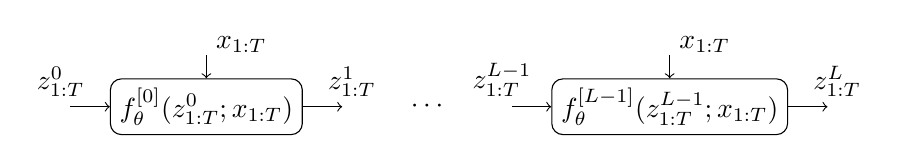
\begin{tikzpicture}[node distance = 0.3cm and 0.5cm, auto, align=center]    
    % blocks
    \node[] (inL1) {};
    \node[block, right= of inL1] (L1) {$f_{\theta}^{[0]}(z_{1:T}^0; x_{1:T})$};
    \node[right= of L1] (outL1) {};
    \node[above= of L1] (inX) {};

    \node[right= of outL1] (dots) {$\cdots$};

    \node[right= of dots] (inLL) {};
    \node[block, right= of inLL] (LL) {$f_{\theta}^{[L-1]}(z_{1:T}^{L-1}; x_{1:T})$};
    \node[right= of LL] (outLL) {};
    \node[above= of LL] (inXL) {};
    
    
    % Input and outputs coordinates
    
    % lines
    \draw[->] (inX) node[right] {$x_{1:T}$} -- (L1.north);
    \draw[->] (inL1) node[above] {$z_{1:T}^0$} -- (L1);
    \draw[->] (L1)  --  (outL1) node[above] {$z^1_{1:T}$};
    \draw[->] (inXL) node[right] {$x_{1:T}$} -- (LL.north);
    \draw[->] (inLL) node[above] {$z_{1:T}^{L-1}$} -- (LL);
    \draw[->] (LL) -- (outLL) node[above] {$z_{1:T}^L$};

\end{tikzpicture}    
        \end{onlyenv}
        \begin{onlyenv}<2-3>
            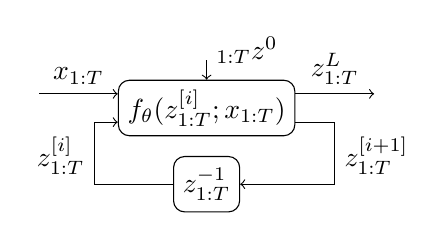
\begin{tikzpicture}[node distance = 0.25cm and 0.5cm, auto, align=center]    
    \node[] (inL) {};
    \node[block, right= of inL] (L) {$f_{\theta}(z_{1:T}^{[i]}; x_{1:T})$};
    \node[right= of L] (outL) {};
    \node[above= of L] (inZ) {};
    \node[block, below= of L] (delay) {$z_{1:T}^{-1}$};

    \coordinate[] (output_zL)  at ($(L.south east)!0.75!(L.north east)$);
    \coordinate[] (output_zi)  at ($(L.south east)!0.25!(L.north east)$);
    \coordinate[] (input_x) at ($(L.south west)!0.75!(L.north west)$);
    \coordinate[] (input_zi) at ($(L.south west)!0.25!(L.north west)$);

    % \draw[->] (inZ) \node[right] {$z^{0}$} -- (L.north);
    \draw[->] (inZ) node[right] {$_{1:T}z^0$} -- (L.north);
    \draw[<-] (input_x) -- node[above] {$x_{1:T}$} ++(-1, 0);
    \draw[->] (output_zL) -- node[above] {$z_{1:T}^L$} ++(1,0);
    \draw[->] (output_zi) -- ++(0.5,0)  |- node[above right] {$z_{1:T}^{[i+1]}$} (delay.east);
    \draw[->] (delay.west) -- ++(-1,0)node[above left] {$z_{1:T}^{[i]}$} |- (input_zi);
    % \draw[->] (output_zi) -- ++(1,0) -| \node[below] {$z^{i+1}$} (input_zi)
\end{tikzpicture}
        \end{onlyenv}
        \begin{onlyenv}<4->
            $\operatorname{RootFind}\left(\underbrace{f_{\theta}(z_{1:T};x_{1:T})- z_{1:T}}_{g_{\theta}}\right)$
        \end{onlyenv}

        
    };
    \node at (G.north) [above] {$\mathcal{S}_{\operatorname{DEQ}}$};
    \node[right= of G] (output) {};
    
    % Input and outputs coordinates
    
    % lines
    \draw[->] (input)  node[above] {$x_{1:T}, z_{1:T}^0$} -- (G);
    \begin{onlyenv}<1-3>
        \draw[->] (G) -- (output) node[above] {$z_{1:T}^L$} ;    
    \end{onlyenv}
    \begin{onlyenv}<4->
        \draw[->] (G) -- (output) node[above] {$z_{1:T}^*$} ;    
    \end{onlyenv}
    

\end{tikzpicture}
    \end{figure}

    \begin{onlyenv}<3->
        \begin{block}{Core idea of \glspl{deq}}
            \begin{itemize}
                \item What happens for $L\to\infty$?
                \begin{onlyenv}<4->
                    $$z_{1:T}^* = f_{\theta}(z_{1:T}^*;x_{1:T})$$
                \end{onlyenv}
                \begin{onlyenv}<5->
                \item How restrictive is weight tying?
                \begin{onlyenv}<6->
                    \begin{itemize}
                        \item \emph{... Any traditional $L$-layer deep network (in "standard" format) can be represented by a weight-tied, input-injected network of equivalent depth, with linear increase in width ...}
                    \end{itemize}    
                \end{onlyenv}
                
                \end{onlyenv}
                \begin{onlyenv}<7->
                \item Any \emph{black-box-root-finding} algorithm can be applied to solve the forward pass
                \end{onlyenv}
                
                % \item  Equilibrium point $z_{1:T}^* = f_{\theta}(z_{1:T}^*;x_{1:T})$
                % \item Find equilibrium point via root finding method e.g. \emph{Newton's method}
                %     \begin{equation}
                %         \label{eq:root_find}
                %         z_{1:T}^* = \operatorname{RootFind}(g_{\theta}; x_{1:T}),
                %     \end{equation}
                %     were $g_{\theta}(z_{1:T}^{*}; x_{1:T}) = f_{\theta}(z_{1:T}^{*}; x_{1:T})-z_{1:T}^*$
                % \item No gradients on each layer, classical backpropagation not possible.
            \end{itemize}
        \end{block}
    \end{onlyenv}
    
\end{frame}

\subsection{Backward Pass}
\begin{frame}{\Acrlong{deq} - Backward Pass}
    \framesubtitle{\cite{bai2019deep}}
    \begin{columns}[T]
        \column{0.5\textwidth}
            \textbf{Traditional backpropagation is not suitable}
                \begin{itemize}
                    \item Would depend on the root finding method
                    \item Intermediate results are not stored during the forward pass
                \end{itemize}
        \column{0.5\textwidth}
        \begin{onlyenv}<1>
            \begin{figure}
                
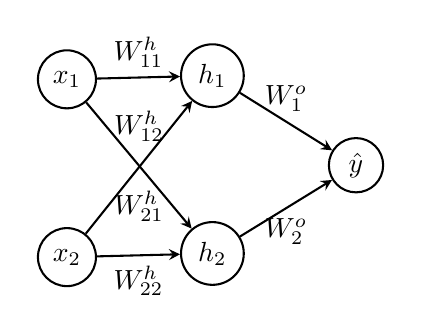
\begin{tikzpicture}[>=stealth,->,line width=0.75pt]
    
    \matrix[matrix of nodes, column sep=3em, row sep=1em, align=center, nodes={rectangle, anchor=center}, every node/.style = {draw, shape=circle, align=center},] {
        \node (x1) {$x_1$}; & \node (h1) {$h_1$};\\
        & & \node (o) {$\hat{y}$}; \\
        \node (x2) {$x_2$}; & \node (h2) {$h_2$};\\
    };
    
    \draw (x1) -> (h1) node[above,midway] {$W^{\text{h}}_{11}$};
    \draw (x1) -> (h2) node[above,midway,yshift=0.5em] {$W^{\text{h}}_{12}$};
    \draw (x2) -> (h1) node[below,midway,yshift=-0.5em] {$W^{\text{h}}_{21}$};
    \draw (x2) -> (h2) node[below,midway] {$W^{\text{h}}_{22}$};
    \draw (h1) -> (o) node[above,midway] {$W^{\text{o}}_{1}$};
    \draw (h2) -> (o) node[below,midway] {$W^{\text{o}}_{2}$};
\end{tikzpicture}
                \caption{Backpropagation usually takes the same route as the forward pass.}
            \end{figure}
        \end{onlyenv}

        
    \end{columns}
    \begin{onlyenv}<2->
        \begin{block}{Gradient of the Equilibrium Model}
            Assume the loss function
             $$\ell=\mathcal{L}\left(h\left(\operatorname{RootFind}\left(g_0 ; x_{1:T}\right)\right), y_{1: T}\right)$$
            \begin{itemize}
                \item $h:\mathbb{R}^{n_z} \mapsto \mathbb{R}^{n_y}$ can be any differentiable function (e.g. linear)
                \item $y_{1:T}$ is the ground-truth sequence
                \item $\mathcal{L}:\mathbb{R}^{n_y}\times\mathbb{R}^{n_y} \mapsto \mathbb{R}$ is the loss function
            \end{itemize}
            \begin{onlyenv}<3->
                The loss gradient with respect to $(\cdot)$ is
                $$\frac{\partial \ell}{\partial(\cdot)}=-\frac{\partial \ell}{\partial h} \frac{\partial h}{\partial z}_{1: T}^{\star}\left(\left.J_{g_\theta}^{-1}\right|_{{x}_{1: T}^*}\right) \frac{\partial f_\theta\left(z_{1: T}^{\star} ; x_{1: T}\right)}{\partial(\cdot)}$$
                \begin{itemize}
                    \item $\left.J_{g_\theta}^{-1}\right|_{{x}_{1: T}^*}$ si the inverse Jacobian of $g_{\theta}$ evaluated at $x$
                \end{itemize}
            \end{onlyenv}
        \end{block}
    \end{onlyenv}

    
\end{frame}

\defverbatim[colored]\makeFwd{
\begin{lstlisting}[language=Python, style=numbered, caption={Traditional forward pass},label=code:fwd]
# forward pass for fixed number of layers
z = torch.zeros(size=(1, n_z))
x = torch.tensor(u).reshape(1, n_x)
for l in range(L):
    z = nl(W_z(z) + U_z(x))
y_hat = W_y(z)
\end{lstlisting}
}
\defverbatim[colored]\makeDeq{
\begin{lstlisting}[language=Python, style=numbered, caption={Forward pass of \gls{deq}},label=code:deq]   
# DEQ
def g_theta(z):
    z = z.reshape(n_z,1)
    return np.squeeze(np.tanh(W_z_numpy @ z + U_z_numpy @ x + b_z_numpy) - z)

z_star, infodict, ier, mesg = fsolve(g_theta, x0=z_0, full_output=True)
z_star = z_star.reshape(n_z, 1)
y_hat_eq = W_y_numpy @ z_star + b_y_numpy
\end{lstlisting}
}
\defverbatim[colored]\makeCmp{
\begin{lstlisting}[language=Python, style=numbered,label=code:cmp]  
Number of finite layers: 0       || z^L - z^* ||^2: 0.7032
Number of finite layers: 1       || z^L - z^* ||^2: 0.3898
Number of finite layers: 2       || z^L - z^* ||^2: 0.2898
Number of finite layers: 3       || z^L - z^* ||^2: 0.1621
Number of finite layers: 4       || z^L - z^* ||^2: 0.09451
Number of finite layers: 10      || z^L - z^* ||^2: 0.001685
Number of finite layers: 20      || z^L - z^* ||^2: 7.595e-06
Number of finite layers: 30      || z^L - z^* ||^2: 7.069e-08
\end{lstlisting}
}
\subsection{Example}
\begin{frame}{Simple \gls{deq} - Example}
    \vspace{-0.5cm}
    \textbf{\emph{Assume}: Sequence length $T=3$, size of hidden state $n_z = 10$, input and output size $n_y = n_x = 1$}:
    \begin{itemize}
        \item Weights are randomly initialized
        \item Initial hidden state $z^0_{1:T} = 0$
        \item $W_z \in \mathbb{R}^{n_z \times n_z}$, $U_z\in \mathbb{R}^{n_z \times T}$
        \item Linear output layer $W_y \in \mathbb{R}^{n_y \times n_z}$
    \end{itemize}
    \vspace{0.2cm}
    \begin{columns}
        \column{0.5\textwidth}
        \begin{onlyenv}<2,4->
            \textbf{Network with fixed layer size:}
            $$
                \begin{aligned}
                    z_{1:T}^{l+1} & = \sigma\left(W_z z_{1:T}^{l} + U_z x_{1:T} + b_z\right) \qquad l=1, \ldots, L-1\\
                    \hat{y}_{1:T} & = W_y z^*_{1:T} + b_z
                \end{aligned}
            $$
        \end{onlyenv}

        \column{0.5\textwidth}
        \begin{onlyenv}<3->
            \textbf{\Gls{deq}:}
            $$
                \begin{aligned}
                    z_{1:T}^{*} & = \operatorname{RootFind}\left(\sigma\left(W_z z_{1:T} + U_z x_{1:T} + b_z\right)- z_{1:T}\right)\\
                    \hat{y}_{1:T} & = W_y z^L_{1:T} + b_z
                \end{aligned}
            $$
        \end{onlyenv}

    \end{columns}
    \begin{onlyenv}<2>

        \makeFwd
    \end{onlyenv}
    \begin{onlyenv}<3>
        \makeDeq
    \end{onlyenv}
    \begin{onlyenv}<4->
        \vspace{0.2cm}
        \textbf{Comparison:}
            \makeCmp
    \end{onlyenv}
\end{frame}

\defverbatim[colored]\makeInit{
\begin{lstlisting}[language=Python, style=numbered, caption={Added line $2$}, label=code:init]  
W_z = torch.nn.Linear(in_features=n_z, out_features=n_z, bias=True)
torch.nn.init.normal_(W_z.weight)
U_z = torch.nn.Linear(in_features=n_x, out_features=n_z, bias=False)
W_y = torch.nn.Linear(in_features=n_z, out_features=n_x, bias=True)
\end{lstlisting}
}
\defverbatim[colored]\makeCmpMon{
\begin{lstlisting}[language=Python, style=numbered, label=code:cmp2]  
    Number of finite layers: 0       || z^L - z^* ||^2: 0.4664
    Number of finite layers: 1       || z^L - z^* ||^2: 0.332
    Number of finite layers: 2       || z^L - z^* ||^2: 1.035
    Number of finite layers: 3       || z^L - z^* ||^2: 1.834
    Number of finite layers: 4       || z^L - z^* ||^2: 2.348
    Number of finite layers: 10      || z^L - z^* ||^2: 2.75
    Number of finite layers: 20      || z^L - z^* ||^2: 2.724
    Number of finite layers: 30      || z^L - z^* ||^2: 2.927
\end{lstlisting}
}


\section{\Acrlongpl{mondeq}}
\subsection{Motivation}
\begin{frame}{Example continued}
    \textbf{Do the solutions $z^{*}_{1:T}$ and $z^L_{1:T}$ always converge for sufficient large $L$?}
    \begin{itemize}
        \item Let the weight of the hidden layer be initialized by a normal distribution
    \end{itemize}
    \makeInit
    \pause
    \textbf{Comparison}:
    \makeCmpMon
\end{frame}
\subsection{Formal Definition}
\begin{frame}{Core idea of \acrfull{mondeq}}
    \framesubtitle{\cite{winston2020monotone}}
    \vspace{-0.5cm}
    \begin{block}{Finding equilibrium point as operator splitting \cite[Theorem 1]{winston2020monotone}}
        Consider (again) a weight-tied input-injected network
        \begin{equation}
            z^{k+1} = \sigma\left(W_z z^k + U_z x+b_z\right)
            \label{eq:iter}
        \end{equation}
        and an equilibrium point that remains constant after update
        $$
            z^* = \sigma\left(Wz_z^* + U_zx+b\right).
        $$
        Finding an equilibrium point of \eqref{eq:iter} is equivalent of finding a zero of the operator splitting problem $0 \in (F+G)(z^*)$ with the operators
        \begin{equation}
            F(z) = (I-W_z)(z) - (U_z x+b), \qquad G=\partial f
            \label{eq:operator_splitting}
        \end{equation}
        and $\sigma(\cdot) = \operatorname{prox}_f^1(\cdot)$ for some convex closed proper function $f$, where $\operatorname{prox}_f^{\alpha}$ denotes the proximal operator
        $$
            \operatorname{prox}_f^{\alpha}(x) \equiv \operatorname{argmin}_z \frac{1}{2}\|x - z\|_2^2 + \alpha f(z)
        $$
    \end{block}
    \pause
    \begin{itemize}
        \item An introduction to monotone operator theory would be required to fully appreciate the result, see \cite[Appendix A]{winston2020monotone}
        \item Lets view the operator splitting as a \emph{black-box-root-finding} algorithm
    \end{itemize}
\end{frame}

\defverbatim[colored]\makeDeqUniform{
\begin{lstlisting}[language=Python, style=numbered, label=code:deqUniform]  
min EW of (I-W_z): 0.6272        L: 40   || z^L - z^* ||^2: 3.999e-08
min EW of (I-W_z): 0.3782        L: 40   || z^L - z^* ||^2: 4.184e-08
min EW of (I-W_z): 0.5671        L: 40   || z^L - z^* ||^2: 3.373e-08
min EW of (I-W_z): 0.6786        L: 40   || z^L - z^* ||^2: 6.231e-08
min EW of (I-W_z): 0.8057        L: 40   || z^L - z^* ||^2: 2.551e-08
min EW of (I-W_z): 0.662         L: 40   || z^L - z^* ||^2: 3.364e-08
min EW of (I-W_z): 0.3946        L: 40   || z^L - z^* ||^2: 4.522e-08
min EW of (I-W_z): 0.6532        L: 40   || z^L - z^* ||^2: 2.656e-08
min EW of (I-W_z): 0.4264        L: 40   || z^L - z^* ||^2: 3.059e-08
min EW of (I-W_z): 0.6787        L: 40   || z^L - z^* ||^2: 5.395e-08
\end{lstlisting}
}
\defverbatim[colored]\makeDeqNormal{
\begin{lstlisting}[language=Python, style=numbered, label=code:deqNormal]  
min EW of (I-W_z): -2.172        L: 40   || z^L - z^* ||^2: 3.301
min EW of (I-W_z): -2.353        L: 40   || z^L - z^* ||^2: 2.48
min EW of (I-W_z): -1.519        L: 40   || z^L - z^* ||^2: 2.585
min EW of (I-W_z): -1.657        L: 40   || z^L - z^* ||^2: 2.839
min EW of (I-W_z): -0.6791       L: 40   || z^L - z^* ||^2: 2.59
min EW of (I-W_z): -2.574        L: 40   || z^L - z^* ||^2: 3.095
min EW of (I-W_z): -1.609        L: 40   || z^L - z^* ||^2: 3.514
min EW of (I-W_z): -3.02         L: 40   || z^L - z^* ||^2: 2.832
min EW of (I-W_z): -1.922        L: 40   || z^L - z^* ||^2: 2.983
min EW of (I-W_z): -1.023        L: 40   || z^L - z^* ||^2: 2.722
\end{lstlisting}
}
\subsection{Existence of a unique solution}
\begin{frame}{Monotone Operator}
    \vspace{-0.5cm}
    \begin{block}{Monotone operator $F(z) = (I-W_z)(z)- (U_z x+b)$ from \eqref{eq:operator_splitting}.}
        If 
        $$
            I-W_z \succeq mI \qquad m>0
        $$
        is strongly monotone, an unique equilibrium point $z^*$ exists.
    \end{block}
    \begin{itemize}
        \item For a scalar, linear function this connection is intuitive
        $$
            F_{\operatorname{scal}}(z) = \underbrace{(1-w)}_{\text{slope}}z + \underbrace{(ux+b)}_{\text{constant}}
        $$ 
    \end{itemize}
    \begin{onlyenv}<2>
        \makeDeqUniform
    \end{onlyenv}
    \begin{onlyenv}<3>
        \makeDeqNormal
    \end{onlyenv}

    \begin{onlyenv}<4->
        \begin{block}{Introduce constraints on the weight $W_z$ to ensure montonicity}
            Monotonicity is ensured $I-W_z\succeq mI$ if there exists $A,~B \in \mathbb{R}^{n_z \times n_z}$ such that
            $$
                W_z = (1-m)I - A^{\mathrm{T}}A+B-B^{\mathrm{T}}.
            $$
        \end{block}
        \begin{itemize}
            \item The weight $W_z$ is now directly parametrized by $A$ and $B$
        \end{itemize}
    \end{onlyenv}
        
\end{frame}


\section{Connection to System Theory}
\subsection{Nonlinear system identification}
\begin{frame}{Inverted pendulum with torque input}
    \framesubtitle{Classical toy example in control}
    \begin{columns}[]
        \column{0.6\textwidth}      
        % \textbf{Difference equation of pendulum dynamics}
        % \begin{align}
        %     \mathcal{G} &\left\{ \begin{aligned} 
        %         x^{k+1} & = 
        %         \begin{pmatrix}
        %             1 & \delta \\
        %             \frac{g \delta}{l} & 1 - \frac{\mu \delta}{m l^2}
        %         \end{pmatrix}
        %         x^k + 
        %         \begin{pmatrix}
        %             0 \\
        %             -\frac{g\delta}{l}
        %         \end{pmatrix}
        %         u^k +
        %         \begin{pmatrix}
        %             0 \\
        %             \frac{\delta}{ml^2}
        %         \end{pmatrix}
        %         w^k \\
        %         y^k & = 
        %         \begin{pmatrix}
        %             1 & 0
        %         \end{pmatrix} x^k \\
        %         z^k & = 
        %         \begin{pmatrix}
        %             1 & 0
        %         \end{pmatrix}
        %         x^k
        %     \end{aligned} \right.\label{eq:linear_inv_pend}\\
        %     w^k &  = \Delta(z^k) = z^k - \sin(z^k) \label{eq:nonlinear_inv_pend}
        % \end{align}
        \begin{block}{System Identification Problem}
            If the equations of the pendulum are not available but we are given data $\mathcal{D} = \{(u,y)_i\}_i^N$, which contains input output measurements. Finding the parameter set $\theta$ can be seen as a deep learning problem.
        \end{block}
        \begin{itemize}
            \item The system states $x_{\text{sys}}^k = [\phi, ~ \dot{\phi}]^{\mathrm{T}}$ represents the \emph{angle} and \emph{angular velocity}
            \item Input $u^k$ represents a torque
            \item Output $y^k$ is the \emph{angle} $\phi$
            \item One stable and one unstable equilibrium point         
        \end{itemize}
        % \begin{onlyenv}<2>
        %     \begin{block}{}
        %         Linearized system can be used to design a controller that stabilizes the unstable equilibrium point
        %     \end{block}
        % \end{onlyenv}

        % \begin{figure}
        %     \begin{tikzpicture}[node distance = 0.25cm and 0.7cm, auto, align=center]
    % blocks
    \node[] (output) {};
    \begin{onlyenv}<-3>
        \node[block, right= of output] (G) {$\begin{array}{ll}\textcolor{green}{x^{k+1}} & = \textcolor{red}{A}x^k + \textcolor{red}{B_1} u^k+\textcolor{green}{B_2}w^k \\ \hat{y}^k & = \textcolor{red}{C_1}x^k+\textcolor{red}{D_{11}}u^k+ D_{12}w^k\\ z^k & = C_2\textcolor{green}{x^k}+D_{21}u^k \end{array}$};
        % Input and outputs coordinates
        \coordinate[] (outputz)  at ($(G.south west)!0.75!(G.north west)$);
        \coordinate[] (outputy)  at ($(G.south west)!0.25!(G.north west)$);
        \coordinate[] (inputw) at ($(G.south east)!0.75!(G.north east)$);
        \coordinate[] (inputu) at ($(G.south east)!0.25!(G.north east)$);
        \node[right= of G] (input) {};
        \node[block, above= of G] (delta) {$w^k = \Delta(z^k)$};    
        % lines
        \draw[<-] (inputu) --  node[above right ] {$u^k$} ++(1,0);
        \draw[->] (outputz)node[above left]{$z^k$}  -- ++(-0.5,0) |-   (delta.west) ;
        \draw[->] (outputy)  -- node[above left] {$\hat{y}^k$} ++(-1,0);
        \draw[->] (delta.east)  -- ++(2,0) |- node[above right] {$w^k$}(inputw) ;
    \end{onlyenv}
    \begin{onlyenv}<4>
        \node[block, right= of output] (G) {$\begin{array}{ll}h^{(t)} & = I w^k \\ \hat{y}^k & = D_{12}w^k\\ z^k & = C_2h^{(t-1)}+D_{21}u^k \end{array}$};
        % Input and outputs coordinates
        \coordinate[] (outputz)  at ($(G.south west)!0.75!(G.north west)$);
        \coordinate[] (outputy)  at ($(G.south west)!0.25!(G.north west)$);
        \coordinate[] (inputw) at ($(G.south east)!0.75!(G.north east)$);
        \coordinate[] (inputu) at ($(G.south east)!0.25!(G.north east)$);
        \node[right= of G] (input) {};
        \node[block, above= of G] (delta) {$w^k = \tanh(z^k)$};    
        % lines
        \draw[<-] (inputu) --  node[above right ] {$u^k$} ++(1,0);
        \draw[->] (outputz)node[above left]{$z^k$}  -- ++(-0.5,0) |-   (delta.west) ;
        \draw[->] (outputy)  -- node[above left] {$\hat{y}^k$} ++(-1,0);
        \draw[->] (delta.east)  -- ++(1.5,0) |- node[above right] {$w^k$}(inputw) ;
    \end{onlyenv}

\end{tikzpicture}
        %     \caption{LTI system in feedback interconnection with nonlinearity}
        % \end{figure}
        \column{0.4\textwidth}
        \vspace{-0.7cm}
        % \begin{onlyenv}<1>
        \movie[autostart]{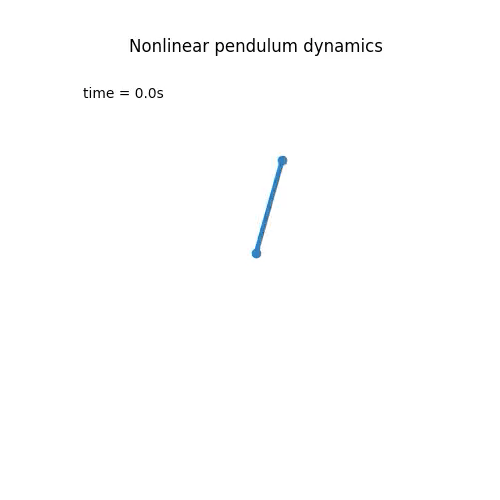
\includegraphics[width=\textwidth]{inv_pendulum_poster.png}}{./fig/inv_pendulum.mov}    
        % \end{onlyenv}
        % \begin{onlyenv}<2>
        %     \movie[autostart]{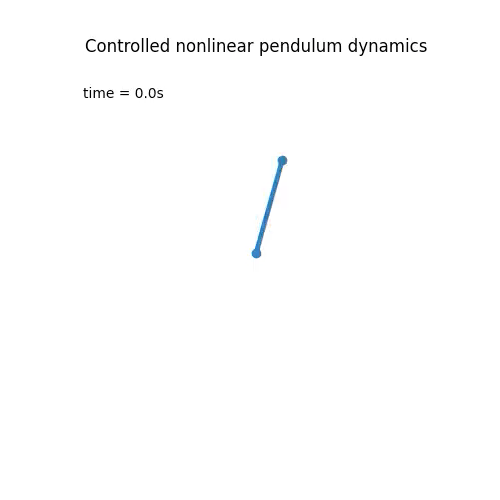
\includegraphics[width=\textwidth]{inv_pendulum_controlled_poster.png}}{./fig/inv_pendulum_controlled.mov}  
        % \end{onlyenv}
        
        \vspace{-0.7cm}
        \begin{figure}
            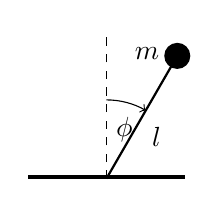
\begin{tikzpicture}[auto, node distance=1.8cm]
 
    % Support
    \fill (-1,0) rectangle(1,0.05);
     
    % Bob's trajectory
    \draw[<-] (60:1) arc(60:90:1);
     
    % Rod + Bob
    \draw[thick] (0,0) -- (60:0.9)node[anchor=north west](l){$l$} -- (60:1.6) node[anchor=south east]{$m$} -- (60:1.8) node[fill, circle]{};
     
     
    % Light gray pendulum
    \draw[dashed] (0,0) -- (90:0.9) node[anchor=north west]{$\phi$} -- (90:1.8) node[]{};
     
\end{tikzpicture}
            \caption{Parameters of single pendulum.}
        \end{figure}
    \end{columns}

\end{frame}

\subsection{Recurrent Neural Networks as \gls{lti} system}
\begin{frame}{Generalization of Recurrent Neural Networks}
    \framesubtitle{LTI system with nonlinear disturbance}
    \vspace{-0.5cm}
    \begin{columns}
        \column{0.5\textwidth}
        \begin{onlyenv}<1->
            \begin{figure}
                \centering
                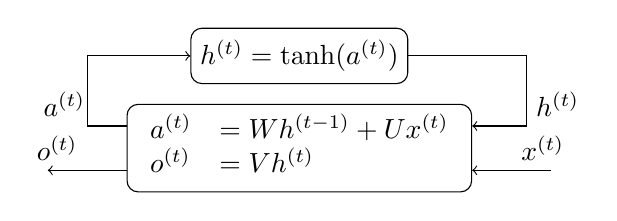
\begin{tikzpicture}[node distance = 0.25cm and 0.5cm, auto, align=center]    
    % blocks
    \node[] (output) {};
    \node[block, right= of output] (G) {$\begin{array}{ll}a^{(t)} & = W h^{(t-1)} + Ux^{(t)} \\
o^{(t)} & = V h^{(t)}\end{array}$};
    \node[block, above= of G] (delta) {$h^{(t)} = \tanh(a^{(t)})$};
    \node[right= of G] (input) {};
    
    % Input and outputs coordinates
    \coordinate[] (outputz)  at ($(G.south west)!0.75!(G.north west)$);
    \coordinate[] (outputy)  at ($(G.south west)!0.25!(G.north west)$);
    \coordinate[] (inputw) at ($(G.south east)!0.75!(G.north east)$);
    \coordinate[] (inputu) at ($(G.south east)!0.25!(G.north east)$);
    
    % lines
    \draw[<-] (inputu) --  node[above right ] {$x^{(t)}$} ++(1,0);
    \draw[->] (outputz) -- ++ (-0.4,0) node[above left]{$a^{(t)}$}  -- ++(-0.1,0) |-   (delta.west) ;
    \draw[->] (outputy)  -- node[above left] {$o^{(t)}$} ++(-1,0);
    \draw[->] (delta.east)  -- ++(1.5,0) |- node[above right] {$h^{(t)}$}(inputw) ;
\end{tikzpicture}
                \caption{Recurrent neural network from \cite{goodfellow2016deep}}
                \label{fig:rnn}
            \end{figure}
        \end{onlyenv}
    
        \column{0.5\textwidth}
        \begin{onlyenv}<2->
            \begin{figure}
                \centering
                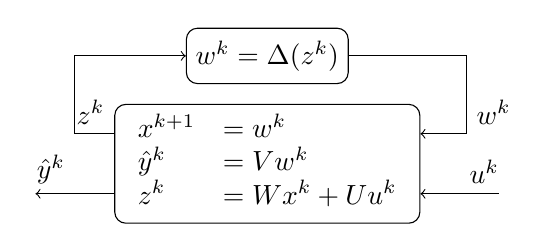
\begin{tikzpicture}[node distance = 0.25cm and 0.5cm, auto, align=center]        
        % blocks
        \node[] (output) {};
        \node[block, right= of output] (G) {$\begin{array}{ll}x^{k+1} & = w^k \\
    \hat{y}^k & =V w^k \\ z^k & = W x^k + U u^k\end{array}$};
        \node[block, above= of G] (delta) {$w^k = \Delta(z^k)$};
        \node[right= of G] (input) {};
        
        % Input and outputs coordinates
        \coordinate[] (outputz)  at ($(G.south west)!0.75!(G.north west)$);
        \coordinate[] (outputy)  at ($(G.south west)!0.25!(G.north west)$);
        \coordinate[] (inputw) at ($(G.south east)!0.75!(G.north east)$);
        \coordinate[] (inputu) at ($(G.south east)!0.25!(G.north east)$);
        
        % lines
        \draw[<-] (inputu) --  node[above right ] {$u^k$} ++(1,0);
        \draw[->] (outputz)node[above left]{$z^k$}  -- ++(-0.5,0) |-   (delta.west) ;
        \draw[->] (outputy)  -- node[above left] {$\hat{y}^k$} ++(-1,0);
        \draw[->] (delta.east)  -- ++(1.5,0) |- node[above right] {$w^k$}(inputw) ;
    \end{tikzpicture}
                \caption{Using common notation from system theory.}
                \label{fig:rnn_intermediate}
            \end{figure}
        \end{onlyenv}
    \end{columns}

    \begin{onlyenv}<3->
        \begin{figure}
            \centering
            \label{fig:lti_cmp}
            \begin{tikzpicture}[node distance = 0.25cm and 0.7cm, auto, align=center]
    % blocks
    \node[] (output) {};
    \begin{onlyenv}<-3>
        \node[block, right= of output] (G) {$\begin{array}{ll}\textcolor{green}{x^{k+1}} & = \textcolor{red}{A}x^k + \textcolor{red}{B_1} u^k+\textcolor{green}{B_2}w^k \\ \hat{y}^k & = \textcolor{red}{C_1}x^k+\textcolor{red}{D_{11}}u^k+ D_{12}w^k\\ z^k & = C_2\textcolor{green}{x^k}+D_{21}u^k \end{array}$};
        % Input and outputs coordinates
        \coordinate[] (outputz)  at ($(G.south west)!0.75!(G.north west)$);
        \coordinate[] (outputy)  at ($(G.south west)!0.25!(G.north west)$);
        \coordinate[] (inputw) at ($(G.south east)!0.75!(G.north east)$);
        \coordinate[] (inputu) at ($(G.south east)!0.25!(G.north east)$);
        \node[right= of G] (input) {};
        \node[block, above= of G] (delta) {$w^k = \Delta(z^k)$};    
        % lines
        \draw[<-] (inputu) --  node[above right ] {$u^k$} ++(1,0);
        \draw[->] (outputz)node[above left]{$z^k$}  -- ++(-0.5,0) |-   (delta.west) ;
        \draw[->] (outputy)  -- node[above left] {$\hat{y}^k$} ++(-1,0);
        \draw[->] (delta.east)  -- ++(2,0) |- node[above right] {$w^k$}(inputw) ;
    \end{onlyenv}
    \begin{onlyenv}<4>
        \node[block, right= of output] (G) {$\begin{array}{ll}h^{(t)} & = I w^k \\ \hat{y}^k & = D_{12}w^k\\ z^k & = C_2h^{(t-1)}+D_{21}u^k \end{array}$};
        % Input and outputs coordinates
        \coordinate[] (outputz)  at ($(G.south west)!0.75!(G.north west)$);
        \coordinate[] (outputy)  at ($(G.south west)!0.25!(G.north west)$);
        \coordinate[] (inputw) at ($(G.south east)!0.75!(G.north east)$);
        \coordinate[] (inputu) at ($(G.south east)!0.25!(G.north east)$);
        \node[right= of G] (input) {};
        \node[block, above= of G] (delta) {$w^k = \tanh(z^k)$};    
        % lines
        \draw[<-] (inputu) --  node[above right ] {$u^k$} ++(1,0);
        \draw[->] (outputz)node[above left]{$z^k$}  -- ++(-0.5,0) |-   (delta.west) ;
        \draw[->] (outputy)  -- node[above left] {$\hat{y}^k$} ++(-1,0);
        \draw[->] (delta.east)  -- ++(1.5,0) |- node[above right] {$w^k$}(inputw) ;
    \end{onlyenv}

\end{tikzpicture}
            \caption{LTI with nonlinear disturbance.}
        \end{figure}  
        \vspace{-0.3cm}  
        \vfill
        \begin{block}{}
            \begin{itemize}
                \item For $A=B_1=C_1=D_{11}, D_{22} = 0$, $B_2 = I$, $\Delta(\cdot) = \tanh(\cdot)$ and $h^{t-1} = x^k$ the networks in Figure~\ref{fig:rnn} and Figure~8 are equivalent
            \end{itemize}
        \end{block}

    \end{onlyenv}
\end{frame}

\subsection{\Acrlong{ren}}
\begin{frame}{Linear systems with disturbances can be analyzed with tools from robust control}
    \vspace{-0.5cm}
    \begin{onlyenv}<1>
        \begin{columns}
            \column{0.6\textwidth}
                \textbf{Neural networks with guarantees}
                \begin{itemize}
                    \item \Gls{rnn} interpreted as linear systems with nonlinear disturbances can be analyzed with tools from robust control
                    \item The neural network has system theoretic guarantees
                \end{itemize}
            \column{0.4\textwidth}
                \begin{figure}
                    
\includegraphics[width=\textwidth]{ren.png}
                    \caption{From CDC 2021, \emph{about 8 citations}\cite{revay2021recurrent}}
                \end{figure}
        \end{columns}
    \end{onlyenv}
    \begin{onlyenv}<2>
        \begin{figure}
            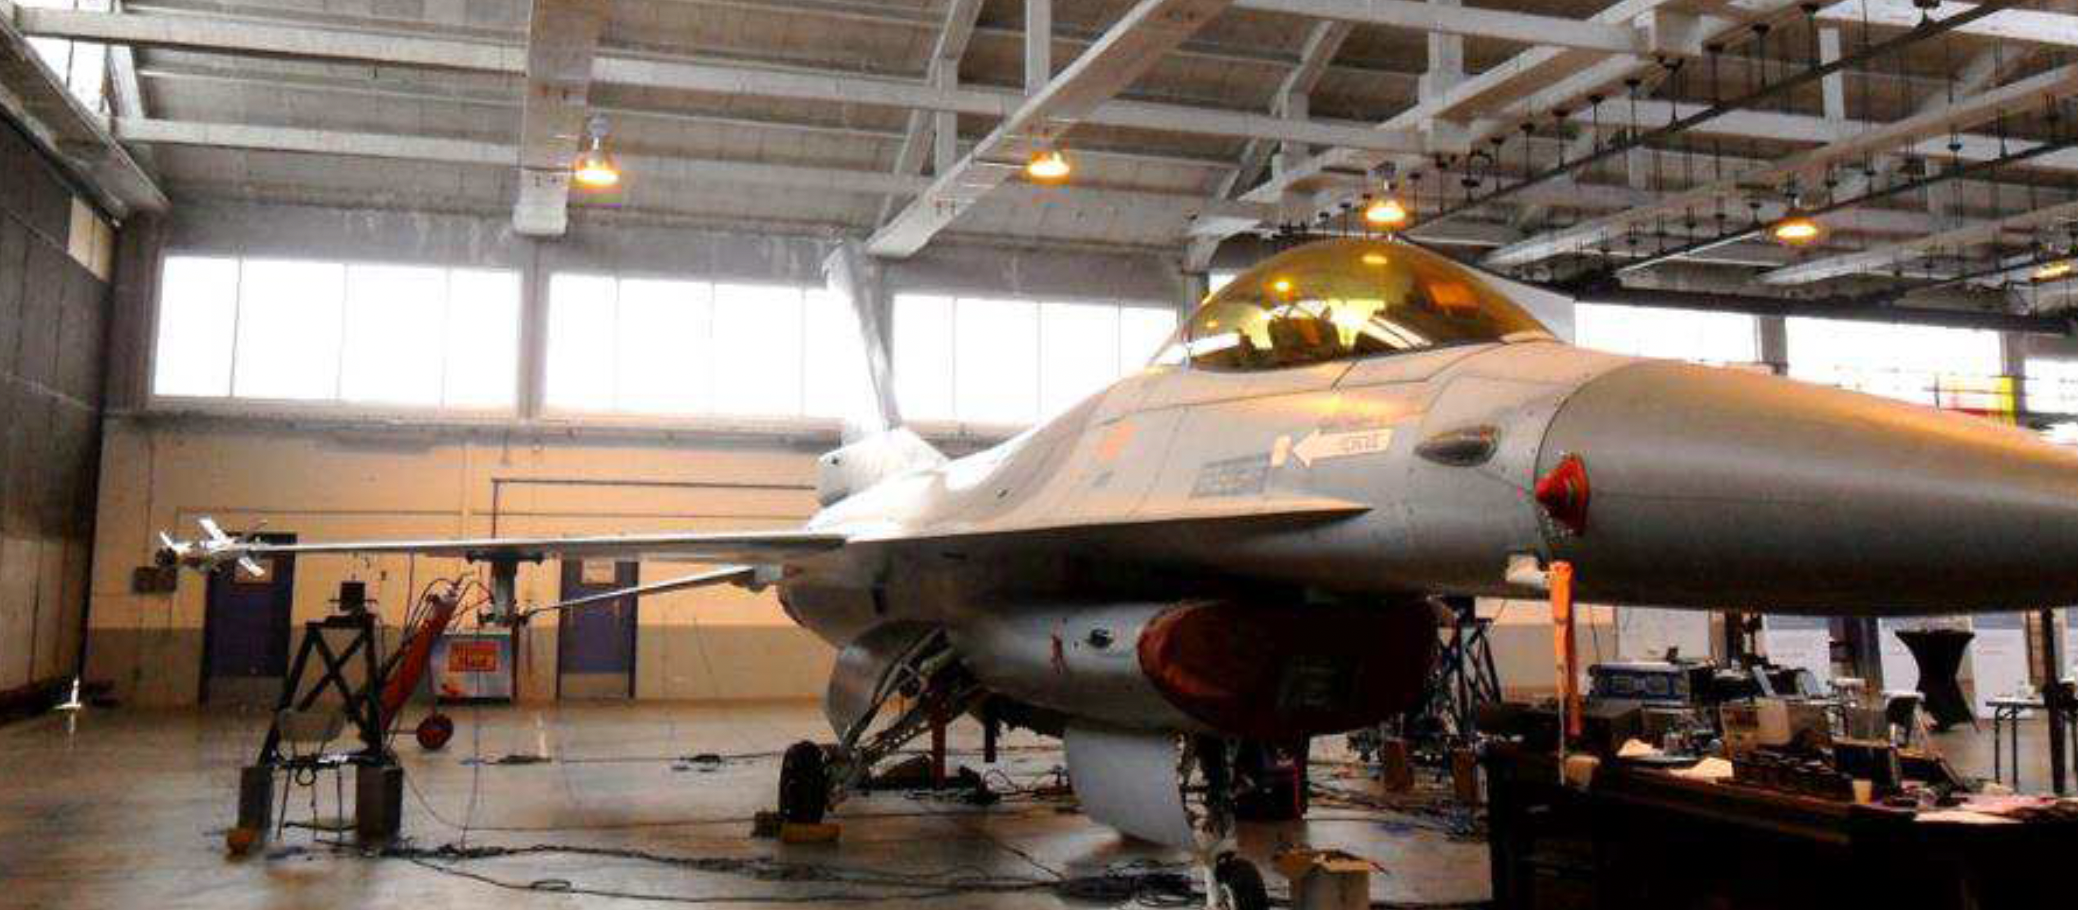
\includegraphics[width=0.4\textwidth]{fig/f16.png}
            \caption{F16 nonlinear system identification benchmark \cite{noel2017f}}
        \end{figure}
        
    \end{onlyenv}
    \begin{onlyenv}<2>
        \begin{columns}[T]
            \column{0.5\textwidth}
                \begin{figure}
                    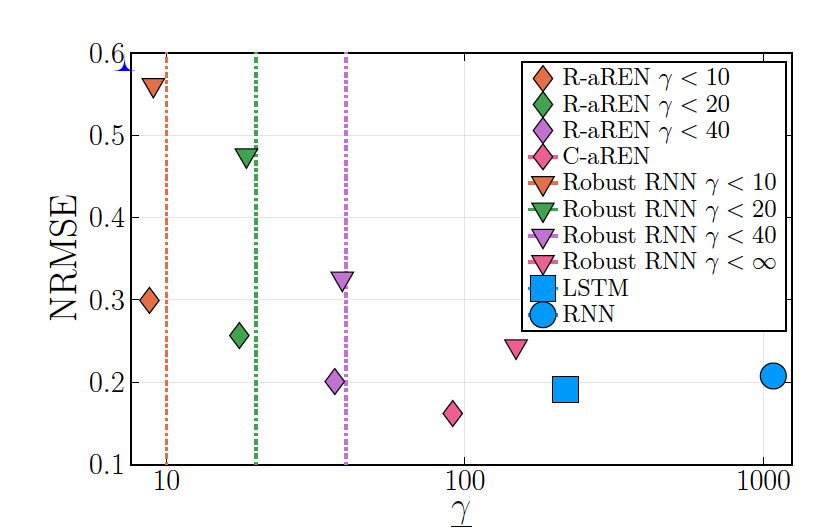
\includegraphics[width=0.75\textwidth]{fig/rob_vs_acc.png}
                    \caption{Robustness versus accuracy \cite[Fig. 2]{revay2021recurrent}}
                \end{figure}
            \column{0.5\textwidth}
                \begin{figure}
                    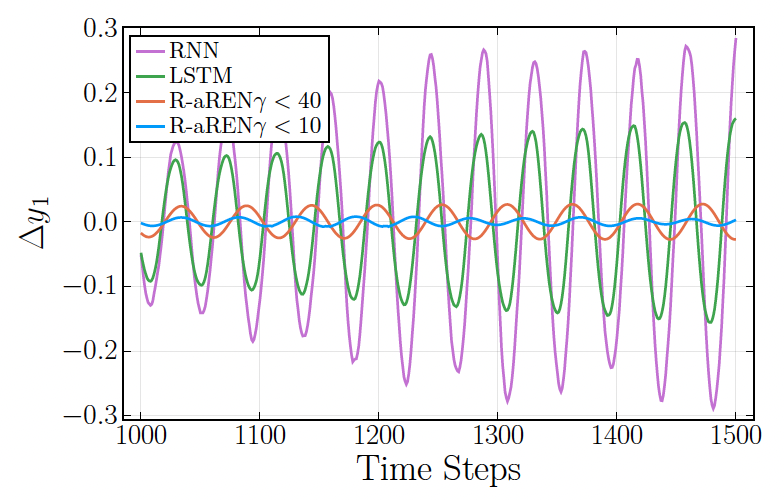
\includegraphics[width=0.75\textwidth]{fig/perf.png}
                    \caption{Stability \cite[Fig. 5]{revay2021recurrent}}
                \end{figure}
        \end{columns}
    \end{onlyenv}
\end{frame}




%%%%%%%%%%%%%%%%%%%%%%%%%%%%%%%%% final slide %%%%%%%%%%%%%%%%%%%%%%%%%%%%%%%%%%
% \finalslide{<<email>>}{<<tel>>}{<<street>>}{<<PLZ City>>}{<<Room>>}{<<department link>>}
\finalslide{daniel.frank@ipvs.uni-stuttgart.de}{+49 711 685-88107}{Universitaetstraße 32}{70569 Stuttgart}{2.204}{https://www.ipvs.uni-stuttgart.de/departments/ac/}

%%%%%%%%%%%%%%%%%%%%%%%%%%%%%%%%%%% appendix %%%%%%%%%%%%%%%%%%%%%%%%%%%%%%%%%%%


\appendix
\begin{frame}[allowframebreaks]{Literature}
  \bibliographystyle{apalike}  
  \bibliography{bib}
\end{frame}



\section{Background}



\begin{frame}{Pendulum is also in LTI structure}
    \framesubtitle{Same representation as RNNs}
    \vspace{-0.2cm}
    \begin{columns}[T]
        \column{0.6\textwidth}      
        \textbf{Difference equation of pendulum dynamics}
        \begin{align*}
            \mathcal{G} &\left\{ \begin{aligned} 
                x^{k+1} & = 
                \underbrace{\begin{pmatrix}
                    1 & \delta \\
                    \frac{g \delta}{l} & 1 - \frac{\mu \delta}{m l^2}
                \end{pmatrix}}_A
                x^k + 
                \underbrace{\begin{pmatrix}
                    0 \\
                    -\frac{g\delta}{l}
                \end{pmatrix}}_{B_1}
                u^k +
                \underbrace{\begin{pmatrix}
                    0 \\
                    \frac{\delta}{ml^2}
                \end{pmatrix}}_{B_2}
                w^k \\
                y^k & = 
                \underbrace{\begin{pmatrix}
                    1 & 0
                \end{pmatrix}}_{C_1} x^k \\
                z^k & = 
                \underbrace{\begin{pmatrix}
                    1 & 0
                \end{pmatrix}}_{C_2}
                x^k
            \end{aligned} \right.\\
            w^k &  = \Delta(z^k) = z^k - \sin(z^k)
        \end{align*}
        \column{0.4\textwidth}
        \begin{figure}
            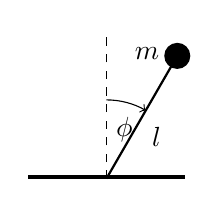
\begin{tikzpicture}[auto, node distance=1.8cm]
 
    % Support
    \fill (-1,0) rectangle(1,0.05);
     
    % Bob's trajectory
    \draw[<-] (60:1) arc(60:90:1);
     
    % Rod + Bob
    \draw[thick] (0,0) -- (60:0.9)node[anchor=north west](l){$l$} -- (60:1.6) node[anchor=south east]{$m$} -- (60:1.8) node[fill, circle]{};
     
     
    % Light gray pendulum
    \draw[dashed] (0,0) -- (90:0.9) node[anchor=north west]{$\phi$} -- (90:1.8) node[]{};
     
\end{tikzpicture}
            \caption{Parameters of single pendulum.}
        \end{figure}
    \end{columns}
    \begin{figure}
        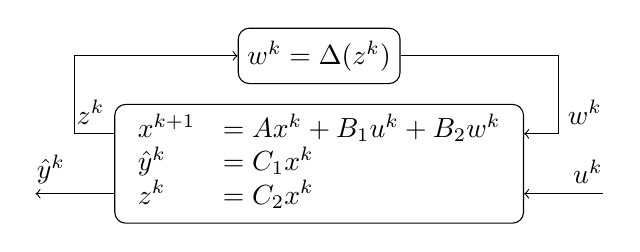
\begin{tikzpicture}[node distance = 0.25cm and 0.7cm, auto, align=center]
    % blocks
    \node[] (output) {};
    \node[block, right= of output] (G) {$\begin{array}{ll}x^{k+1} & = Ax^k + B_1 u^k+B_2w^k \\ \hat{y}^k & = C_1x^k\\ z^k & = C_2x^k \end{array}$};
    \node[right= of G] (input) {};
    \node[block, above= of G] (delta) {$w^k = \Delta(z^k)$};    
    % Input and outputs coordinates
    \coordinate[] (outputz)  at ($(G.south west)!0.75!(G.north west)$);
    \coordinate[] (outputy)  at ($(G.south west)!0.25!(G.north west)$);
    \coordinate[] (inputw) at ($(G.south east)!0.75!(G.north east)$);
    \coordinate[] (inputu) at ($(G.south east)!0.25!(G.north east)$);

    % lines
    \draw[<-] (inputu) --  node[above right ] {$u^k$} ++(1,0);
    \draw[->] (outputz)node[above left]{$z^k$}  -- ++(-0.5,0) |-   (delta.west) ;
    \draw[->] (outputy)  -- node[above left] {$\hat{y}^k$} ++(-1,0);
    \draw[->] (delta.east)  -- ++(2,0) |- node[above right] {$w^k$}(inputw) ;


\end{tikzpicture}
        \caption{Pendulum dynamics in LTI structure with nonlinearity $\Delta(\cdot)$}
    \end{figure}
    
\end{frame}

\begin{frame}{Why is this connection interesting?}
    \begin{columns}
        \column{0.7\textwidth}
        \textbf{Linear systems are well understood}
        \begin{itemize}
            \item Stability depends on eigenvalues of $A$ matrix
            \item Well established controller design techniques
        \end{itemize}

        \column{0.3\textwidth}
        \begin{figure}
            
\includegraphics[width=0.6\textwidth]{lunze.png}
            \caption{\cite{lunze1996regelungstechnik}}
        \end{figure}
    \end{columns}
    \pause
    \begin{columns}
        \column{0.7\textwidth}
        \textbf{Linear system with disturbances}
        \begin{itemize}
            \item For known disturbances robust control methods can be applied
            \item Activation function of neural networks can be seen as disturbance
        \end{itemize}

        \begin{block}{System Identification Problem}
            If the equations of the pendulum are not available but we are given data $\mathcal{D} = \{(u,y)_i\}_i^N$, which contains input output measurements. Finding the parameters $A,B_1,B_2,C_1,C_2$ can be seen as a deep learning problem.
        \end{block}

        \column{0.3\textwidth}
        \begin{figure}
            
\includegraphics[width=0.8\textwidth]{willems.png}
            \caption{\cite{willems1972dissipative}}
        \end{figure}
    \end{columns}
    \pause
    \begin{block}{}
        Neural networks that can be represented in LTI structure with nonlinear disturbances can be analyzed with well established tools from robust control.
    \end{block}
    
\end{frame}

\section{Figures}
\begin{frame}[allowframebreaks]{Figures}
    \begin{figure}
        \documentclass[crop, tikz, convert={outfile=.svg}]{standalone}

\usepackage{tikz}
\usetikzlibrary{matrix,shapes,arrows,positioning,chains,patterns,fit,decorations.pathreplacing,calc,plotmarks}
\tikzset{
    dotted_block/.style={
        draw=black!30!white, 
        dashed,
        inner ysep=2mm,
        inner xsep=10mm, 
        rectangle, 
        rounded corners
    },
    block/.style={
        draw,
        rectangle,
        rounded corners,
        minimum height=2em,
        minimum width=2em
    },
    operator/.style={
        draw,
        circle,
        thin,
        minimum height=1em,
	   inner sep=1pt
    },
    weight/.style={
        draw,
        thin,
        rounded corners,
        rectangle,
        %minimum height=2em,
        %minimum width=4em
    },
    value/.style={
        draw,
        thin,
        rectangle,
        %minimum height=2em,
        %minimum width=3em
    },
    gain/.style={
        regular polygon, 
        regular polygon sides=3,
        draw, 
        fill=white, 
        text width=1em,
        inner sep=1mm, 
        outer sep=0mm,
        shape border rotate=-90
    },
    concat/.style={
        draw,
        shape=circle, 
        fill=black,
        %minimum height=0.5em,
	   inner sep=0pt
    },
}
\usepackage{amsfonts}       % blackboard math symbols
\usepackage{amsmath,amssymb}

\begin{document}

\begin{tikzpicture}[node distance = 0.25cm and 0.5cm, auto, align=center]    
    % blocks
    \node[] (input) {};
    \node[block, right= of input] (G) {
        \begin{tikzpicture}[node distance = 0.1cm and 0.5cm, auto, align=center]    
            % blocks
            \node[] (inL1) {};
            \node[block, right= of inL1] (L1) {$f_{\theta}^{[0]}(x^0; u)$};
            \node[right= of L1] (outL1) {};
            \node[above= of L1] (inX) {};
        
            \node[right= of outL1] (dots) {$\cdots$};
        
            \node[right= of dots] (inLL) {};
            \node[block, right= of inLL] (LL) {$f_{\theta}^{[L-1]}(x^{L-1}; u)$};
            \node[right= of LL] (outLL) {};
            \node[above= of LL] (inXL) {};
            
            
            % Input and outputs coordinates
            
            % lines
            \draw[->] (inX.center) node[above] {$u$} -- (L1.north);
            \draw[->] (inL1.center) node[left] {$x^0$} -- (L1);
            \draw[->] (L1.east)  --  (outL1.center) node[right] {$x^1$};
            \draw[->] (inXL.center) node[above] {$u$} -- (LL.north);
            \draw[->] (inLL.center) node[left] {$x^{L-1}$} -- (LL);
            \draw[->] (LL.east) -- (outLL.center) node[right] {$x^L$};
        
        \end{tikzpicture} 
    };
    % \node at (G.north) [above] {$\mathcal{S}_{\operatorname{DEQ}}$};
    \node[right= of G] (output) {};
    
    % Input and outputs coordinates
    
    % lines
    \draw[->] (input)  node[left] {$u, x^0$} -- (G);
    \draw[->] (G) -- (output) node[right] {$x^L$} ;    
    
\end{tikzpicture}

\end{document}
    \end{figure}

    \begin{figure}
        \documentclass[crop, tikz, convert={outfile=.svg}]{standalone}

\usepackage{tikz}
\usetikzlibrary{matrix,shapes,arrows,positioning,chains,patterns,fit,decorations.pathreplacing,calc,plotmarks}
\tikzset{
    dotted_block/.style={
        draw=black!30!white, 
        dashed,
        inner ysep=2mm,
        inner xsep=10mm, 
        rectangle, 
        rounded corners
    },
    block/.style={
        draw,
        rectangle,
        rounded corners,
        minimum height=2em,
        minimum width=2em
    },
    operator/.style={
        draw,
        circle,
        thin,
        minimum height=1em,
	   inner sep=1pt
    },
    weight/.style={
        draw,
        thin,
        rounded corners,
        rectangle,
        %minimum height=2em,
        %minimum width=4em
    },
    value/.style={
        draw,
        thin,
        rectangle,
        %minimum height=2em,
        %minimum width=3em
    },
    gain/.style={
        regular polygon, 
        regular polygon sides=3,
        draw, 
        fill=white, 
        text width=1em,
        inner sep=1mm, 
        outer sep=0mm,
        shape border rotate=-90
    },
    concat/.style={
        draw,
        shape=circle, 
        fill=black,
        %minimum height=0.5em,
	   inner sep=0pt
    },
}
\usepackage{amsfonts}       % blackboard math symbols
\usepackage{amsmath,amssymb}

\begin{document}

\begin{tikzpicture}[node distance = 0.25cm and 0.5cm, auto, align=center]    
    % blocks
    \node[] (input) {};
    \node[block, right= of input] (G) {
        \begin{tikzpicture}[node distance = 0.25cm and 0.5cm, auto, align=center]    
            \node[] (inL) {};
            \node[block, right= of inL] (L) {$f_{\theta}(x^{[i]}; u)$};
            \node[right= of L] (outL) {};
            \node[above= of L] (inZ) {};
            \node[block, below= of L] (delay) {delay};
        
            \coordinate[] (output_zL)  at ($(L.south east)!0.75!(L.north east)$);
            \coordinate[] (output_zi)  at ($(L.south east)!0.25!(L.north east)$);
            \coordinate[] (input_x) at ($(L.south west)!0.75!(L.north west)$);
            \coordinate[] (input_zi) at ($(L.south west)!0.25!(L.north west)$);
        
            % \draw[->] (inZ) \node[right] {$z^{0}$} -- (L.north);
            \draw[->] (inZ.center) node[above] {$x^0$} -- (L.north);
            \draw[<-] (input_x) -- ++(-1, 0) node[left] {$u$};
            \draw[->] (output_zL) --  ++(1,0) node[right] {$x^L$};
            \draw[->] (output_zi) -- ++(0.5,0)  |- node[above right] {$x^{[i+1]}$} (delay.east);
            \draw[->] (delay.west) -- ++(-1,0)node[above left] {$x^{[i]}$} |- (input_zi);
            % \draw[->] (output_zi) -- ++(1,0) -| \node[below] {$z^{i+1}$} (input_zi)    
        \end{tikzpicture}
    };
    % \node at (G.north) [above] {$\mathcal{S}_{\operatorname{DEQ}}$};
    \node[right= of G] (output) {};
    
    % Input and outputs coordinates
    
    % lines
    \draw[->] (input)  node[left] {$u, x^0$} -- (G);
    \draw[->] (G) -- (output) node[right] {$x^L$} ;    
    
\end{tikzpicture}

\end{document}
    \end{figure}

    \begin{figure}
        \documentclass[crop, tikz, convert={outfile=.svg}]{standalone}

\usepackage{tikz}
\usetikzlibrary{matrix,shapes,arrows,positioning,chains,patterns,fit,decorations.pathreplacing,calc,plotmarks}
\tikzset{
    dotted_block/.style={
        draw=black!30!white, 
        dashed,
        inner ysep=2mm,
        inner xsep=10mm, 
        rectangle, 
        rounded corners
    },
    block/.style={
        draw,
        rectangle,
        rounded corners,
        minimum height=2em,
        minimum width=2em
    },
    operator/.style={
        draw,
        circle,
        thin,
        minimum height=1em,
	   inner sep=1pt
    },
    weight/.style={
        draw,
        thin,
        rounded corners,
        rectangle,
        %minimum height=2em,
        %minimum width=4em
    },
    value/.style={
        draw,
        thin,
        rectangle,
        %minimum height=2em,
        %minimum width=3em
    },
    gain/.style={
        regular polygon, 
        regular polygon sides=3,
        draw, 
        fill=white, 
        text width=1em,
        inner sep=1mm, 
        outer sep=0mm,
        shape border rotate=-90
    },
    concat/.style={
        draw,
        shape=circle, 
        fill=black,
        %minimum height=0.5em,
	   inner sep=0pt
    },
}
\usepackage{amsfonts}       % blackboard math symbols
\usepackage{amsmath,amssymb}

\begin{document}

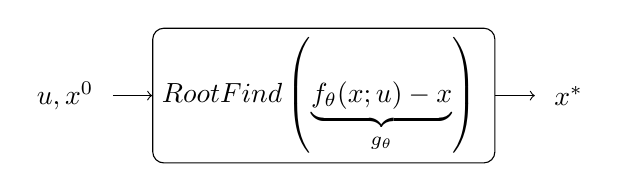
\begin{tikzpicture}[node distance = 0.25cm and 0.5cm, auto, align=center]    
    % blocks
    \node[] (input) {};
    \node[block, right= of input] (G) {
        $\operatorname{RootFind}\left(\underbrace{f_{\theta}(x;u)- x}_{g_{\theta}}\right)$        
    };
    % \node at (G.north) [above] {$\mathcal{S}_{\operatorname{DEQ}}$};
    \node[right= of G] (output) {};
    
    % Input and outputs coordinates
    
    % lines
    \draw[->] (input)  node[left] {$u, x^0$} -- (G);
    \draw[->] (G) -- (output) node[right] {$x^*$} ;    

    

\end{tikzpicture}

\end{document}
    \end{figure}
    
\end{frame}


\subsection{Deep equilibrium model}
    % \begin{itemize}
    %     \item New model architecture for deep sequence models of the form 
    %     \begin{equation}
    %         \label{eq:nonlinear_system}
    %         z_{1:T}^{[i+1]}=f_{\theta}^{[i]}(z_{1:T}^{[i]};x_{1:T}) \text{ for } i=0,1, \ldots, L-1.
    %     \end{equation}
    %     \item input sequence: $x_{1:T} = [x_1, \ldots, x_T] \in \mathbb{R}^{T\times p}$ where $x_i \in \mathbb{R}^p$, $T\in\mathbb{N}$ is the sequence length
    %     \item Find fixed point $z_{1:T}^*$ of nonlinear system \eqref{eq:nonlinear_system} such that $z_{1:T}^* = f_{\theta}(z_{1:T}^*;x_{1:T})$
    %     \item Fix point $z_{1:T}^*$ is the same solution as the forward pass of a deep sequence model.
    %     \item Weights are tied.
    %     \item Consider models that converge to an equilibrium point, output of DEQ is this equilibrium point.
    %     \item Find equilibrium point via root finding method e.g. \emph{Newton's method}
    %     \begin{equation}
    %         \label{eq:root_find}
    %         z_{1:T}^* = \operatorname{RootFind}(g_{\theta}; x_{1:T})
    %     \end{equation}
    %     Were $g_{\theta}(z_{1:T}^{*}; x_{1:T}) = f_{\theta}(z_{1:T}^{*}; x_{1:T})-z_{1:T}^*$
    %    
    %     \begin{itemize}
    %         \item Gradient of equilibrium model (with respect to the parameters $\theta$) can be computed in one step with the Jacobian at equilibrium.
    %     \end{itemize}
    %     \item $f_{\theta}$ needs to be stable and constrained
    % \end{itemize}

% \begin{frame}{Recurrent Equilibrium Models}
%     \framesubtitle{\cite{revay2021recurrent}}
    
% \end{frame}

\end{document}
